\chapter{緒言}

\section{研究背景}
油圧アクチュエータは電動アクチュエータと比べ,外力に対する耐衝撃性・質量出力比・最大出力の大きさ・設計の自由度の高さなどに優れており,現在においても使われる分野は多い.
特に建設機械(耐衝撃性や最大出力)や航空機(質量出力比)などの分野では欠かせないものとなっている.
一方で,油漏れを防ぐためのシーリングによる摩擦や,油自身の圧縮性・温度依存性・発火性など,油圧システム特有の性質に起因する制御性能の低さ,そして電動アクチュエータの高性能化により,一般の機械分野では制御性能に優れる電動のものが使われている.

ところが近年,電動と油圧を組み合わせた電気油圧式アクチュエータの登場や,計算機能力および制御技術の向上により,ロボティクスの分野を中心に油圧アクチュエータが見直されている\cite{feng2014optimization,kuindersma2016optimization,玄相昊2015招待講演}.
油圧アクチュエータを用いるロボットの一つが\figname\ref{fig:PA-2000}に示す6軸油圧マニピュレータPA-2000\cite{IRID}であり,本研究の制御対象である.

PA-2000は福島第一原子力発電所の廃炉に向けて燃料デブリを取り出すために,国際原子炉開発機構(IRID)および三菱重工株式会社により開発試作されているマニピュレータである\cite{河西賢一2018福島第一原子力発電所燃料デブリ横取り出しに向けたロボット開発}.
格納容器内に溶融した状態で存在しているとされる燃料デブリを取り出すためには,狭い通路\footnote{CRD交換用開口を通過する.そのため,PA-2000では外形寸法が\SI{700}{mm}$\times$\SI{920}{mm}に抑えられている.}を通過すること,デブリに対する加工反力に耐えることなどの条件を満たす必要があり,質量出力比に優れる油圧アクチュエータが採用されている.
また,デブリを加工・ハンドリングするなどの操作を行うため,マニピュレータ先端に取り付けるツールは適宜取り替えられる.
原子炉内での燃料デブリ取り出しは,人が立ち入れない高放射線環境下で行われる.
そして放射性物質が漏れ出ないように安全に作業を進めるためには,マニピュレータ先端の位置および力を正確にかつ確実に制御する必要がある.
本研究ではこのうち,手先が対象物に接触している状態において発生させる力を制御することに取り組む.

力を制御するにあたり,手先にかかる力を何らかの方法で取得してフィードバックをする必要がある.
本研究の特徴は,手先にかかる力を直接取り付けたセンサにより取得するのではなく,シリンダに取り付けた圧力センサ情報から間接的に推定することを考える.
力センサを用いないことで,マニピュレータ全体の省線化が図れるとともに,複数種類利用することが想定される先端ツールの設計簡略化が期待される.
また,圧力をフィードバックすることにより,マニピュレータ先端が対象物体に触れたときの姿勢に依らず力を推定できることが期待される.

圧力から力を推定する手法は,佐藤ら\cite{佐藤有香理2015油圧ショベルにおけるバケット先端の負荷力推定}がショベルにおいてなぞり作業時の負荷推定を行い,岡田ら\cite{岡田大貴2016多自由度油圧駆動ロボットのシリンダ圧に基づく手先負荷力推定,岡田大貴2017多自由度油圧駆動ロボットのシリンダ圧に基づく手先負荷力推定による力覚フィードバック}は建設機械ベースのロボットにおいて力覚フィードバックを行っている.
これらの研究ではシリンダから発生する力は圧力と受圧面積から求め,摩擦については触れられていない.
本研究では,システム同定を活用することにより摩擦の影響も含めたモデルを得ることで,より現実に近いシリンダ出力を推定する.
さらに,推定した出力をもとに,力制御系の設計を行う.

\begin{figure}[t]
    \centering
        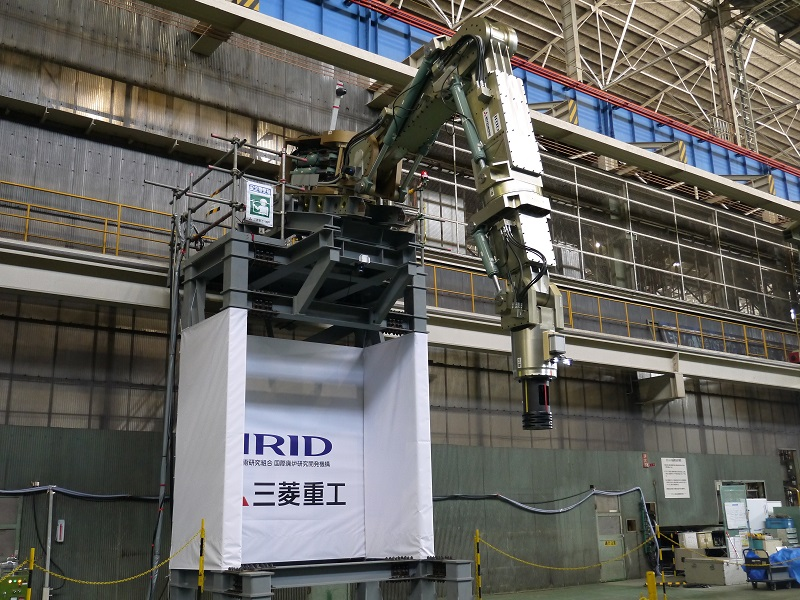
\includegraphics[keepaspectratio, width = .8\linewidth]{contents/緒言/figure/PA-2000.jpg}
        \caption{6-axis Hydraulic Manipulator: PA-2000}
        \label{fig:PA-2000}
\end{figure}

\section{力制御に向けたアプローチ}
力制御に向けたアプローチの概要を\figname\ref{fig:approach_thiswork}に示す.
最終目的の制御対象はPA-2000であるが,大学の研究室レベルにおいてはPA-2000と同じ間接配置を持つマニピュレータORION-7Pを用いて手先での力の推定手法および力制御手法の構築を行うことを目標としている.
本研究では,第一段階として,油圧シリンダ単体を対象として力を推定する手法の構築および推定した力を用いたシリンダの力制御を行う.


\begin{figure}[t]
    \centering
        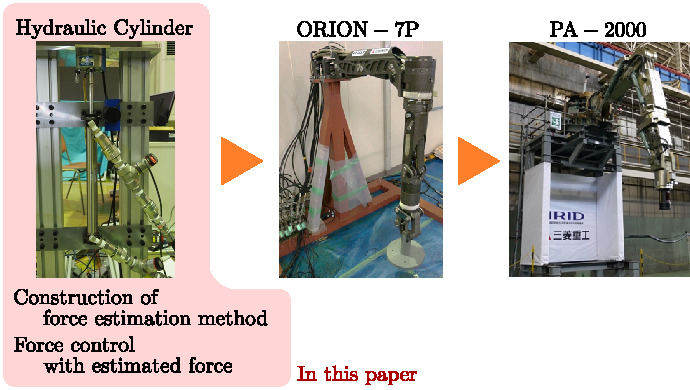
\includegraphics[keepaspectratio, scale=1.0]{contents/緒言/figure/approach_thiswork.pdf}
        \caption{Approach in this work}
        \label{fig:approach_thiswork}
\end{figure}

\section{油圧システムの特徴と関連研究}
本節では,油圧システムの特徴について述べ,油圧アクチュエータ制御の関連研究について紹介する.
\subsection{油圧システムの特徴}

油圧システムの駆動における基本原理はパスカルの原理\cite{PascalsLaw}であり,圧力発生源および圧力を伝える媒体があればアクチュエータを作動させることが可能である.
そのため,電動機の登場以前より重要な駆動力として扱われてきた.
油圧システムの利点を以下に示す\cite{jelali2012hydraulic,不二越ハイドロニクスチーム199305}.
\begin{itemize}
    \item 出力重量比(出力密度)が大きい.
    \item 最大出力が大きく,無段階で出力・速度を設定可能.
    \begin{itemize}
        \item 出力は受圧面積と圧力で決まるため,これらを変えることで出力および動作速度を設定することが可能である.
    \end{itemize}
    \item 外部からの衝撃に頑健であり,過負荷に対する保護が容易である.
    \begin{itemize}
        \item ギヤなどのかみ合わせ部品がなく,衝撃を面で受けるため耐衝撃性が高い.また,一定以上の圧力を逃す構造にすることで過負荷に対して装置本体を守ることができる.
    \end{itemize}
    \item 設計の自由度が高い.
    \begin{itemize}
        \item ホースなどが通るスペースさえあれば,圧力供給源とアクチュエータを離れたところに配置することが可能である.
    \end{itemize}
\end{itemize}

一方,欠点も存在し,その代表的なものを以下に示す.
\begin{itemize}
    \item シーリングが必須であり,それによる摩擦が存在する.
    \item 油の圧縮性や温度依存性がある.
    \item 油への異物混入に弱い.
    \item 油漏れのさいに火災の恐れがある.
\end{itemize}
摩擦や圧縮性などは,スティックスリップなどの非線形性をもたらしており,制御を難しくする要因となっている\cite{松崎淳1962直動形油圧駆動機構におけるスティックスリップ,de1995new}.


\subsection{油圧制御の関連研究}
油圧アクチュエータ制御にについて,モデル化を含め位置制御および力制御において様々な手法の適用・提案がされている.
油圧システムの同定はバルブへの指令電圧を入力,位置を出力としたものについていくつか行われており,Lingらは線形システムとみなしての同定を行い,3次の離散システムでモデル化できることを示している\cite{ling2012system}.前島らは,第一原理に基づくモデルおよび各パラメータの同定\cite{前島祐三2011,前島祐三2014}行っている.
Zulfmanらは,同定を行ったモデルに対しファジィ制御を適用し,位置制御の改善をしている\cite{zheng2009application}.

位置制御においては摩擦補償の適用が行われている\cite{jianyong2012robust,rahmat2011modeling,lischinsky1999friction}.
特に,Rahmatらは摩擦と油の内部漏れを統合して扱い,これらを補償することで性能向上を図っている\cite{rahmat2011modeling}.
また,力制御については,AlleyneらやKoivumakiらの研究があるが,位置制御と比べて数が少ないのが現状である\cite{Alleyne,koivumaki2015stability}.
%\subsubsection{油圧アクチュエータ}
%\subsubsection{油圧機械(ロボット,建設機械など)}



\section{本論文の構成}
本論文の構成は次に示す.
\ref{sec:FundamentalEquation}章では,第一原理に基づいたシステムのモデルの記述をする.これはJelaliらの方法\cite{jelali2012hydraulic}に基づき行う.
\ref{sec:SystemIdentification}章では,油圧システムのシステム同定を行い,力推定の準備をし,
\ref{sec:ForceControl}章において力制御を行う.力制御にあたってはPID制御やI-PD制御,$H_\infty$制御を適用し,比較を行う.
\ref{sec:IntegrationControl}章では位置制御と力制御を組み合わせた制御を行い,コンプライアンス制御の適用も試みる.
